\section{\gls{dft}}
\begin{modified}
The \gls{dft} is a powerful tool for analyzing signals in the frequency domain, often used in applications such as signal processing, image analysis, and data compression. Its ability to transform spatial or temporal data into frequency components makes it particularly effective for isolating patterns or removing noise. In this thesis, the \gls{dft} will be used to compress and clean images during the pre-processing phase, which will be discussed in detail in \cref{chap:methodology}.
\end{modified}
\begin{note}
	Nell'introduzione della tesi sarà già accennato cosa è il pre-process a grandi linee. Poi in methodology sarà descritto meglio
\end{note}

\noindent This procedure, known as spectral analysis, makes it possible to study signals, waves, vibrations, sounds and images. In addition to these areas, DFT also has major scientific applications, such as the precise estimation of sunspot cycles, helping to predict and control phenomena such as geomagnetic storms\footnote{For more about geomagnetic storms and them correlation with sunspot, see \url{https://en.wikipedia.org/wiki/Geomagnetic_storm}}.

\subsection{Insights}
\begin{modified}
	The \gls{dft} is a discrete analogue of the \gls{cft}, which represents a function in terms of its frequency components. More rigorously, given a function $f\in L^1(\mathbb{R})$, its Fourier transform is a functional operator, denoted by $\mathcal{F}$, which associates $f$ with its frequency representation:
	\[
		\mathcal{F}(f): \omega \mapsto \int_{\mathbb{R}} e^{-i2\pi \omega x}f(x)\,dx
	\]
	\begin{note}
		La periodicità di $f$ è richiesta solo nelle serie?
	\end{note}

	\noindent By contrast, the Fourier series applies specifically to periodic functions, representing them as an infinite sum of sine and cosine waves with discrete frequencies. In this context, the \gls{dft} can be viewed as a finite approximation of the Fourier series, applied to sampled data over a finite interval.
\end{modified}

\noindent The \textbf{Fourier inversion theorem} states that, if both $f$ and $\mathcal{F}(f)$ belong to $L^1(\mathbb{R})$ (i.e. they are both integrable), then for almost any $x\in\mathbb{R}$ it is possible to recover $f(x)$ via the following inverse relation:
\[
f(x)=\int_{\mathbb{R}}{\mathcal{F}\left(f\right)}(\omega)e^{i2\pi x\omega}\,d\omega
\]
In other words, the Fourier transform and its inverse allow switching back and forth between the time (or space) and frequency domains.

\bigskip
The discrete version of this transform, namely \gls{dft}, is used to analyse signals sampled at regular intervals. Thus, while \gls{cft} works on continuous signals, \gls{dft} applies to finite and discrete signals, making it suitable for digital signal processing.

\noindent To better understand how \gls{dft} gives information about the amplitudes and phases of the different frequencies that make up a sequence, it is useful to introduce the Fourier coefficients. These coefficients make it possible to decompose a data sequence into sinusoids associated with different frequencies.

\begin{modified}
\begin{remark}
	The Fourier coefficients of the sequence $(x_n)_{n=0}^{N-1}$ is a sequence of complex numbers $(X_k)_{k=0}^{N-1}$ such that:
	\begin{equation}
		x_n = \frac{1}{N}\sum_{k=0}^{N-1} X_k e^{i2\pi\frac{k}{N}n}
	\end{equation}

	\noindent In the follow examples, we want show an intuitive relation between Fourier coefficients and them time series. It is very important to interpretate a result of a \gls{dft}.
\end{remark}
\end{modified}

\begin{exempli_gratia}[Amplitude]
	\begin{toReview}
		In this example we understand how the Fourier coefficients determine the amplitude of a frequency.
	\end{toReview}

	\noindent Take a time series consisting of $N$ complex numbers, described by the following coefficients:
	\[
		X_0=0,\;X_1=A,\;X_2=0\;\cdots\;X_{N-2}=0,\;X_{N-1}=A
	\]
	From these coefficients we obtain the time series:
	\[
		x_n = \frac{1}{N}A\left(e^{i2\pi \frac{n}{N}} + e^{i2\pi \frac{n}{N}(N-1)}\right) = \frac{2A}{N}\cos\left(2\pi\frac{n}{N}\right)
	\]
	\begin{modified}
	We note that the series is only a sinusoidal function, with amplitude $\frac{2A}{N}$ and frequency $\frac{2\pi}{N}$.
	\begin{center}
		\centering
		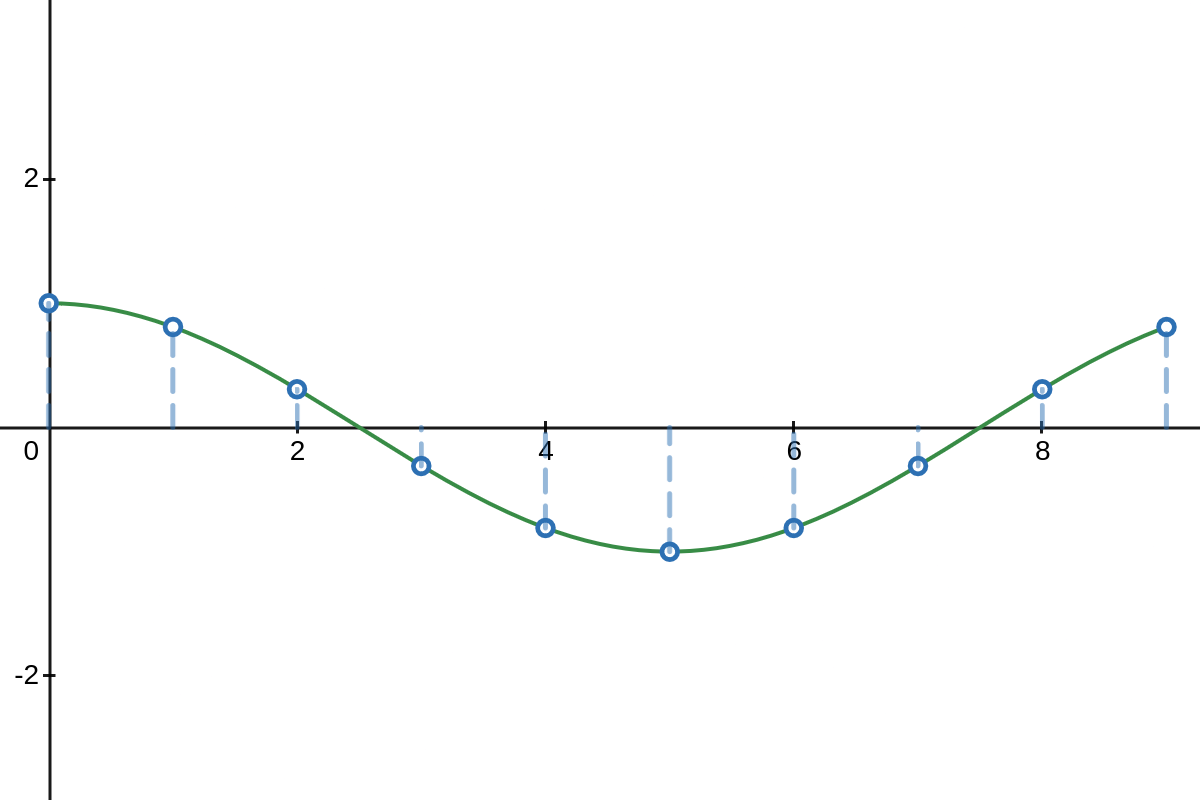
\includegraphics[width=0.5\textwidth]{Figures/fftexample1.png}
	\end{center}
	\end{modified}
\end{exempli_gratia}

\begin{exempli_gratia}[Frequency]
	\begin{toReview}
		In the previous example the significant frequency is $2\pi\frac{n}{N}$, in this example we study how to refer to a different frequency.
	\end{toReview}

	\noindent Take a time series consisting of $N$ complex numbers, described by the following coefficients:
	\[
		X_p=A,\;X_{N-p}=A
	\]
	where all other values are zero.

	\noindent The generated time series will be:
    \[
		x_n = \frac{1}{N}A\left(e^{i2\pi \frac{n}{N}p} + e^{i2\pi \frac{n}{N}(N-p)}\right) = \frac{2A}{N}\cos\left(2\pi\frac{n}{N}p\right)
	\]
	\begin{modified}
	As can be seen, the coefficients refer to the amplitude of a certain frequency indicated by the index of Fourier coefficient.
	\begin{center}
		\centering
		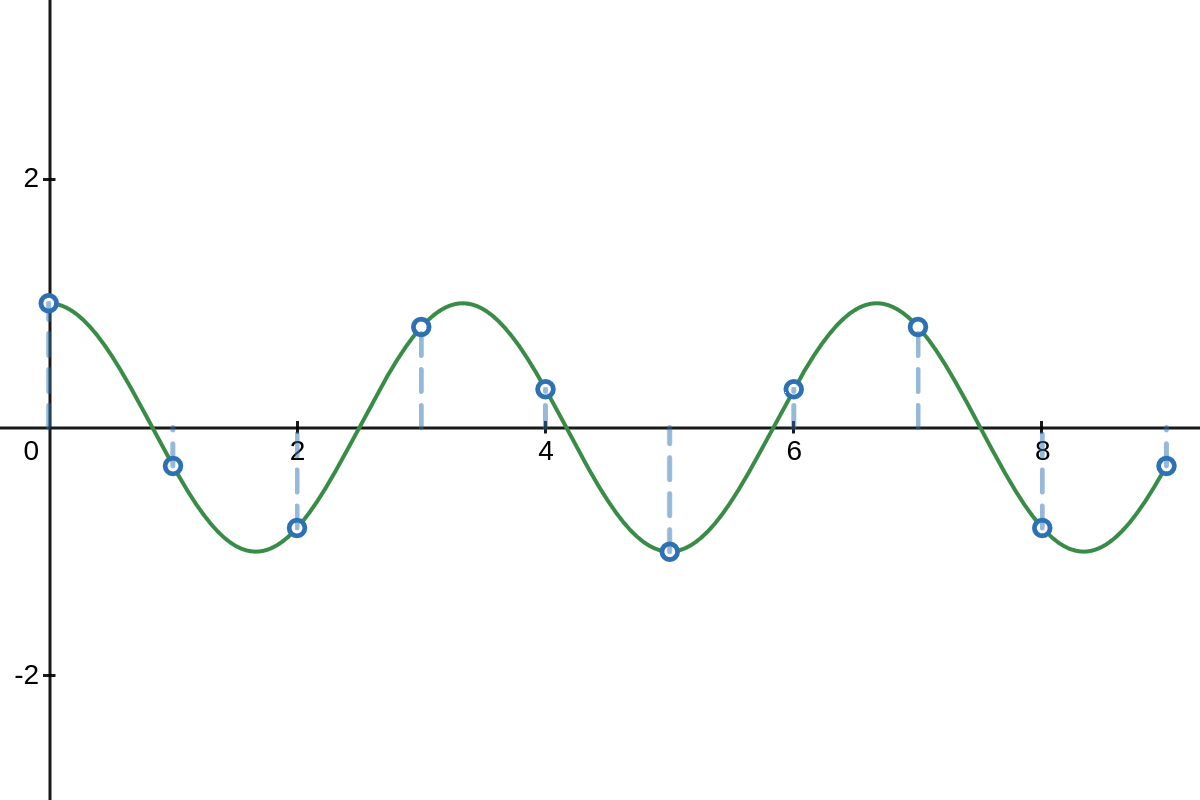
\includegraphics[width=0.5\textwidth]{Figures/fftexample2.png}
	\end{center}

	\noindent If we have $X_1=A, X_{N-1}=A$, $X_2=B, X_{N-2}=B$, then we will obtain time series:
	\[
		x_n = \frac{2A}{N}\cos\left(2\pi\frac{n}{N}\right) + \frac{2B}{N}\cos\left(2\pi\frac{n}{N}2\right)
	\]
	\end{modified}
\end{exempli_gratia}
\begin{exempli_gratia}[Phase]
	\begin{toReview}
		In the previous example we observed that the index of the Fourier coefficient refers to a specific frequency. Now we are going to see how the Fourier coefficients derive the phase of a frequency in a time series.
	\end{toReview}

	\noindent Take a time series consisting of $N$ complex numbers, described by the following coefficients:
	\[
		X_0=0,\;X_1=Ae^{i\theta},\;X_2=0,\;\dots,\;X_{N-2}=0,\;X_{N-1}=Ae^{-i\theta}
	\]
	The resulting time series will be:
    \[
		x_n = \frac{2A}{N}\cos\left(\frac{2\pi}{N}n + \theta\right)
	\]
	Here, the modulus of the coefficient describes the amplitude of the frequency, while its argument $\theta$ describes its phase.
	\begin{center}
		\centering
		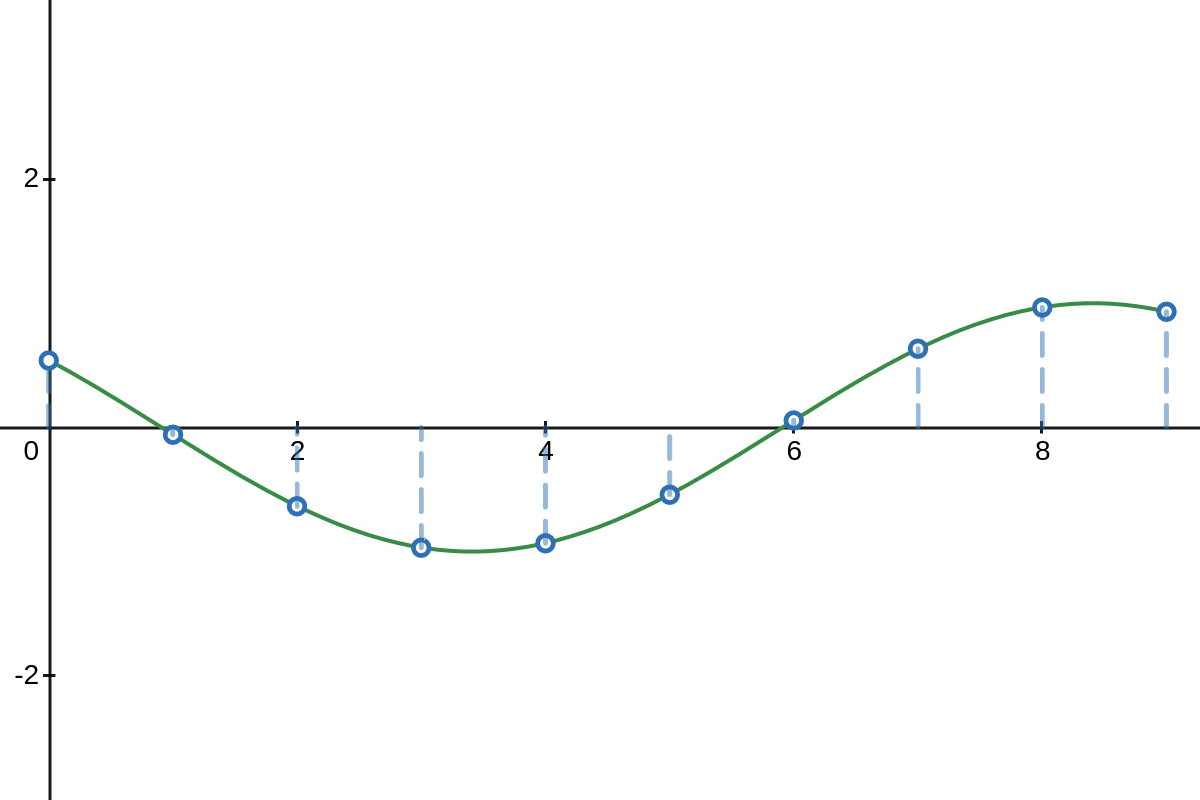
\includegraphics[width=0.5\textwidth]{Figures/fftexample3.png}
	\end{center}

	\begin{modified}
		\noindent We observe also that to ensure that the series is real, the opposite coefficient must be the conjunct of $X_1$.
	\end{modified}
\end{exempli_gratia}

\bigskip
We now ask ourselves whether it is possible to estimate the Fourier coefficients from a time series.
\begin{proposition} \label{prop:dft_unitaria}
	The matrix $\frac{1}{\sqrt{N}}\left(e^{i2\pi\frac{k}{N}n}\right)_{n,k=0}^{N-1}$ is unitary.
	\begin{proof}
		\begin{modified} We prove the thesis by studying the inner product between two rows of the matrix: \end{modified}
		\[
		\frac{1}{N}\sum_{k=0}^{N-1} e^{i2\pi\frac{k}{N}n}\cdot e^{-i2\pi\frac{k}{N}m} = \frac{1}{N}\sum_{k=0}^{N-1} e^{i2\pi\frac{k}{N}(n-m)}
		\]
		If $n = m$, the result of the sum is $1$. Else if $n \neq m$, we obtain:
		\[
			\frac{1}{N}\sum_{k=0}^{N-1} e^{i2\pi\frac{k}{N}(n-m)} = \frac{1}{N}\frac{e^{i2\pi\frac{N}{N}(n-m)}-1}{e^{i2\pi\frac{1}{N}(n-m)}-1} = 0
		\]
		This proves that the matrix is unitary.
	\end{proof}
\end{proposition}

\bigskip
Proving that the matrix $\frac{1}{\sqrt{N}}(e^{i2\pi\frac{k}{N}n})_{n,k=0}^{N-1}$ is unitary is extremely relevant to the computation of Fourier coefficients.
\begin{theorem}[\gls{dft}]
	The Fourier coefficients of the time series $(x_n)_{n=0}^{N-1}$ are given by the formula:
	\begin{equation}
		X_k = \sum_{n=0}^{N-1} x_n e^{-i2\pi\frac{n}{N}k}
	\end{equation}
	\begin{proof}
		Define $U$ as matrix $\frac{1}{\sqrt{N}}(e^{i2\pi\frac{k}{N}n})_{n,k=0}^{N-1}$

		\noindent By definition of the discrete Fourier transform, we can write $\vec{X} = \frac{1}{\sqrt{N}}U\vec{x}$, where $\vec{X}$ is the vector of Fourier coefficients and $\vec{x}$ is the vector of the original time series.

		\noindent As shown in \cref{prop:dft_unitaria}, the matrix $U$ is unitary, so it admits an inverse, which is its transposed conjugate $U^H$. \\
		Therefore, we can invert the transformation and obtain:
		\[
			\vec{x} = \sqrt{N}U^H\vec{X}
		\]

		\noindent This relation allows us to get the Fourier coefficients from the time series.
	\end{proof}
\end{theorem}

\begin{definition}[Fourier coefficient]
	We define Fourier coefficient of the time series $(x_n)^{N-1}_{n=0}$ is the sequence of complex numbers $(X_k)^{N-1}_{k=0}$:
	\[
		X_k = \sum_{n=0}^{N-1} x_n e^{-i2\pi\frac{n}{N}k}
	\]
\end{definition}

\subsection{Implications}
The possibility of calculating Fourier coefficients directly by means of a simple matrix-vector product not only makes the analysis very informative, but also easily achievable.

\begin{modified}
\paragraph{\gls{fft}} The computational cost of the matrix-vector product for computing Fourier coefficients is $O(N^2)$, which is not excessive in itself. However, there are better algorithms that compute Fourier coefficients and that reduce this cost. An example is \gls{czt} algorithm of \citet{czt_source} with computational cost $O(N\log N)$. An other example is the algorithm of \citet{FFT} showed in \cref{alg:fft}, which use a technique of \textit{divide et impera} to compute Fourier coefficients.
\begin{remark}
	The \cref{alg:fft} uses an important property of \gls{fft}: when $N=N_1\times N_2$ with $N_1, N_2> 1$ we can \textit{divide} the input sequence, \textit{impera} over them and, finally, merge results to obtain the desiderate Fourier coefficients.

	\noindent Let $x=(x_i)_{i=0}^{N-1}$ a time series, we compute these Fourier coefficients:
	\begin{itemize}
		\item $X^{0}$ are the Fourier coefficients of  $\left(x_{N_2k}\right)_k$ with $N_1$ values.
		\item $X^{1}$ are the Fourier coefficients of $\left(x_{N_2k+1}\right)_k$ with $N_1$ values.
		\item $\cdots$
		\item $X^{N_2-1}$ are the Fourier coefficients of $\left(x_{N_2k+N_2-1}\right)_k$ with $N_1$ values.
	\end{itemize}
	Now we use them to compute $X$:
	\begin{align*}
		X_k &= \sum_{n=0}^{N-1} x_n e^{-i2\pi\frac{n}{N}k} = \sum_{p=0}^{N_2-1}\sum_{l} x_{N_2l+p} e^{-i2\pi\frac{N_2l+p}{N}k} \\
		&= \sum_{p=0}^{N_2-1}\sum_{l} x_{N_2l+p} e^{-i2\pi\frac{N_2l}{N}k}e^{-i2\pi\frac{p}{N}k} \\
		&= \sum_{p=0}^{N_2-1}e^{-i2\pi\frac{p}{N}k}X^p_k
	\end{align*}
	In particular, the \cref{alg:fft} uses the case of $N_2=2$ and the follow observation:
	\begin{align*}
		X_{k+N/2} &= \sum_{n=0}^{N-1} x_n e^{-i2\pi\frac{n}{N}\left({k+N/2}\right)} = \sum_{n=0}^{N-1} x_n e^{-i2\pi\frac{n}{N}k -i2\pi\frac{n}{2}} \\
		&= \sum_{l} x_{2l} e^{-i2\pi\frac{2l}{N}k -i2\pi l} + \sum_{l} x_{2l} e^{-i2\pi\frac{2l+1}{N}k -i2\pi\frac{2l+1}{2}} \\
		&= X^0_k - e^{-i2\pi\frac{1}{N}k}X^1_k
	\end{align*}
\end{remark}
\noindent The computational cost of \cref{alg:fft} is $O(N\log N)$ if the base case (when $N$ is not even, or in general is a prime) has cost $O(N\log N)$.
\end{modified}

\begin{algorithm}[h]
	\caption[\gls{fft} algorithm]{\citet{FFT} \& \gls{czt} algorithms.\\
		\begin{minipage}[t]{\linewidth}
			\textsc{INPUT}
			\begin{itemize}[noitemsep, topsep=0pt]
				\item[$x$:] time series $x_1,\dots,x_N$
			\end{itemize}
			\textsc{OUTPUT}
			\begin{itemize}[noitemsep, topsep=0pt]
				\item[$X$:] Fourier coefficients of $x$
			\end{itemize}
		\end{minipage}
	}
	\begin{algorithmic}[1]
		\Function{FFT}{$x$}
		\If{$N$ is odd} \Return $\Call{CZT}{x}$ \Comment base case
		\EndIf

		\State $\text{even} \gets \Call{FFT}{\left[x_0,x_2,\cdots,x_{N-2}\right]}$
		\State $\text{odd} \gets \Call{FFT}{\left[x_1,x_3,\cdots,x_{N-1}\right]}$

		\State $X$ is an array of size $N$

		\For{$k\in 0,\dots,\frac{N}{2}-1$}
			\State $t \gets \exp\left(-2\pi i k / N\right)\cdot \text{odd}[k]$
			\State $X[k] \gets \text{even}[k] + t$
			\State $X[k + N/2] \gets \text{even}[k] - t$
		\EndFor
		\State \Return $X$
		\EndFunction
	\end{algorithmic}
	\label{alg:fft}
\end{algorithm}

\begin{modified}
\paragraph{Periodogram} The periodogram is a practical tool that graphically represents the amplitude of the different frequencies composing a time series, providing insight into the frequency spectrum of the signal. By visualising the power associated with each frequency, it highlights the dominant components of the spectrum, making it particularly useful for distinguishing between noise and significant frequencies. This connects directly to the theory of the \gls{dft}, as the periodogram is derived from the squared modulus of the Fourier coefficients, representing the signal's energy distribution across frequencies.

\noindent To illustrate this, we apply the \gls{dft} to the \texttt{sunspots} dataset from the \gls{r} package, which contains the number of sunspots observed each month from $1749$ to $1984$. Sunspots are known to correlate with the Sun's magnetic activity, which is believed to exhibit periodic cycles. Using the periodogram, we aim to identify these cycles, particularly the dominant periodic components in the data, and evaluate their significance compared to noise.
\begin{figure}[ht]
	\centering
	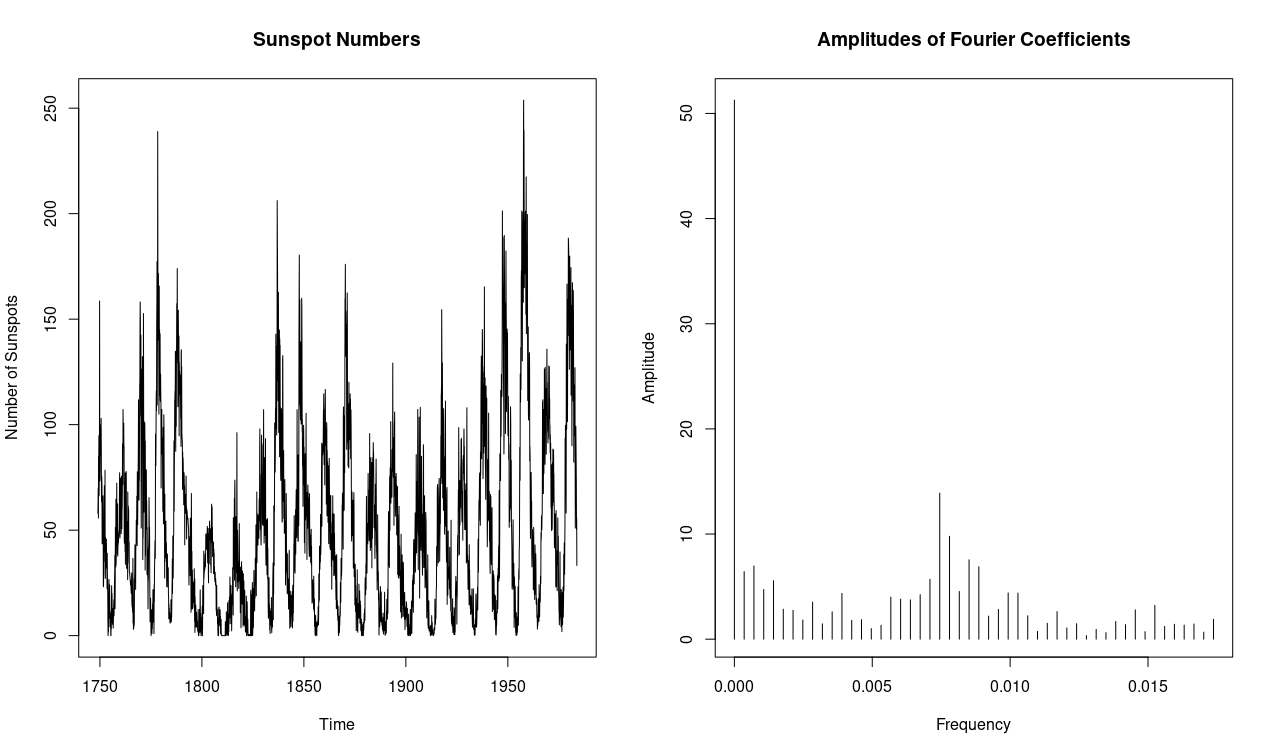
\includegraphics[width=\textwidth]{Figures/sunspots.png}
	\caption[Periodogram of sunspots]{On the left, the time series of the number of sunspots recorded each month from $1749$ to $1984$ (\(N = 2820\)). This representation shows the variation of sunspots over time, highlighting any cycles. On the right, the periodogram obtained by applying the \gls{dft} to the time series. Each point represents the squared modulus of a Fourier coefficient, which measures the energy associated with a given frequency. We can see a peak at frequency $0$, corresponding to the sum of the values of the time series (\(X_0 = \sum_{n=0}^{N-1} x_n\)).}
\end{figure}
\end{modified}

\noindent Looking at the periodogram obtained with \gls{fft}, we observe that some frequencies are much more pronounced than others. In particular, the frequency $\approx 0.0075\operatorname{\mathrm{Hz}}$ (corresponding to about a cycle of $135$ months) indicates a cycle of about $11$ years, which confirms what is already known about the cyclic nature of solar activity.

\noindent This example demonstrates how the DFT is a powerful tool for detecting and analysing periodic patterns in observational data. The use of the periodogram not only makes it possible to identify the main frequencies, but also to evaluate their relative importance respect to the background noise.

\begin{note}
	"Di qual è lo scopo della tesi mi sembra che tu non abbia parlato. Immagino ci sarà nell'introduzione? Ma in ogni caso, in apertura di questo capitolo dovresti anticipare di cosa si parlerà e perché"

	\bigskip \noindent Sì ci sarà nell'introduzione della tesi e ho messo un accenno al suo ruolo nell'introduzione della sezione DFT in queste correzioni
\end{note}
